\documentclass[conference]{IEEEtran}
\IEEEoverridecommandlockouts
% The preceding line is only needed to identify funding in the first footnote. If that is unneeded, please comment it out.
\usepackage{cite}
\usepackage{amsmath,amssymb,amsfonts}
\usepackage{algorithmic}
\usepackage{graphicx}
\usepackage{textcomp}
\usepackage{xcolor}
\usepackage{tabularx}
\usepackage{multirow}
\usepackage{graphics} % for pdf, bitmapped graphics files
\usepackage{subfig}
\usepackage{subcaption}
\usepackage{hyperref}
\usepackage{academicons}
\usepackage{xcolor}
\usepackage{listings}
\def\BibTeX{{\rm B\kern-.05em{\sc i\kern-.025em b}\kern-.08em
		T\kern-.1667em\lower.7ex\hbox{E}\kern-.125emX}}
% Gráficas en MATLAB
\usepackage{tikz, pgfplots}
% Color Enlace
\definecolor{colorEnlace}{RGB}{0, 0, 0}
\hypersetup{
	colorlinks=true,
	linkcolor=colorEnlace,
	citecolor=colorEnlace,
	urlcolor=colorEnlace,
	pdfauthor={Ruth Juana Espino Puma},
	pdftitle={}
}
\lstset{
	language=Matlab, % Define el lenguaje
	basicstyle=\ttfamily\small, % Tamaño de letra pequeño
	keywordstyle=\color{blue}, % Color de las palabras clave
	commentstyle=\color{green}, % Color de los comentarios
	stringstyle=\color{red}, % Color de las cadenas de texto
	numbers=left, % Muestra los números de línea a la izquierda
	numberstyle=\tiny\color{gray}, % Estilo de los números de línea
	tabsize=1,
	stepnumber=1, % Muestra un número en cada línea
	breaklines=true, % Ajuste automático de línea
	frame=single, % Borde alrededor del código
	xleftmargin=0em, % Elimina el margen izquierdo
	framexleftmargin=0em % Elimina el espacio dentro del marco izquierdo
}
% Control 
\usepackage{amsmath}
\begin{document}
	
	\title{Experiencia N°5 - Diseño de Compensadores}
	% Ing. Diego Darcy Arredondo Huarac
	\author{	
		\IEEEauthorblockN{Ruth Juana Espino Puma}
		\IEEEauthorblockA{Universidad Nacional de San Antonio Abad del Cusco}
		\textit{Escuela Profesional de Ingeniería Electrónica}\\
		\textit{Laboratorio de Control I}\\
		184657 \\\\
		Cusco, Perú
	}
	
	\maketitle
	
	\begin{abstract}
		Lead-lag compensators are control systems used to improve the performance and stability of dynamic systems by combining the effects of lead and lag compensators. A lead compensator improves the system’s transient response, reducing overshoot and decreasing the settling time, which is beneficial for systems requiring quick and stable responses. In contrast, a lag compensator primarily improves steady-state accuracy without significant effect on the transient response. When combined in a lead-lag configuration, these compensators help achieve a balanced enhancement, reducing overshoot and achieving desired settling times while maintaining steady-state accuracy and robustness in control systems.
	\end{abstract}
	
	\begin{IEEEkeywords}
		Lead-lag compensator, transient response, settling time, overshoot reduction, steady-state accuracy, control systems, dynamic stability, phase margin, frequency response, system performance
	\end{IEEEkeywords}
	
	\section{Introducción}
	Los compensadores son dispositivos clave en los sistemas de control diseñados para mejorar el rendimiento y la estabilidad de sistemas dinámicos. Estos elementos modifican la respuesta del sistema a través de ajustes en la ganancia y el comportamiento en frecuencia, permitiendo mejorar tanto la precisión en estado estacionario como la respuesta transitoria. Existen diversos tipos de compensadores, como los compensadores de adelanto, que mejoran la respuesta rápida y reducen el tiempo de establecimiento; y los compensadores de atraso, que aumentan la precisión en estado estable sin afectar considerablemente la rapidez. Cuando se combinan en compensadores adelanto-atraso, estos logran un equilibrio, optimizando la estabilidad, reduciendo el sobreimpulso y alcanzando tiempos de respuesta deseados sin comprometer la exactitud en estado estable
	
	\section{Objetivos}
	
	\begin{itemize}
		\item Diseñar Compensadores atraso-adelanto usando el Lugar Geométrico de las Raíces.
		\item Implementar Compensadores atraso-adelanto usando el Lugar Geométrico de las Raíces.
	\end{itemize}
	
	\section{Usando el Lugar Geométrico de las Raíces diseñar compensadores en atraso-adelanto}
	
	El lugar geométrico de las raíces nos permiten conocer la ubicación de los polos de un sistema mediante la variación de un parámetro que normalmente suele ser la ganancia $K$ del sistema, este método además de permitirnos conocer el comportamiento de un sistema para una determinada ganancia según la ubicación de los polos, también brinda un punto de partida para el diseño de compensadores que nos permitan modificar tal respuesta según lo deseado, siendo el caso que para los sistemas:
	
	\begin{itemize}
		\item Sistema subamortiguado se busca reducir el sobreimpulso en un 50\%.
		\item Sistema sobreamortiguado se busca reducir el tiempo de establecimiento a por lo menos la mitad.
	\end{itemize}
	
	Para estos 2 propósitos se busca el diseño e implementación de compensadores en adelanto-atraso, que permitan satisfacer los objetivos para cada sistema.
	
	\subsection{\textbf{Caso Subamortiguado}}
	El sistema subamortiguado tiene la planta definida por la siguiente función de transferencia para los polos ubicados en $S_{1,2} = -10 \pm i15$.
	\begin{equation}
		H(s) = \frac{325}{s^2 + 20s + 325}
		\label{eq:ft-planta}
	\end{equation}
	Para este sistema se busca reducir el sobreimpulso en un 50\% para lo cual se iniciara con el análisis del lugar geométrico del sistema sin compensar que se muestra en la figura \ref{fig:lgrplanta}
	
	\begin{figure}[h]
		\centering
		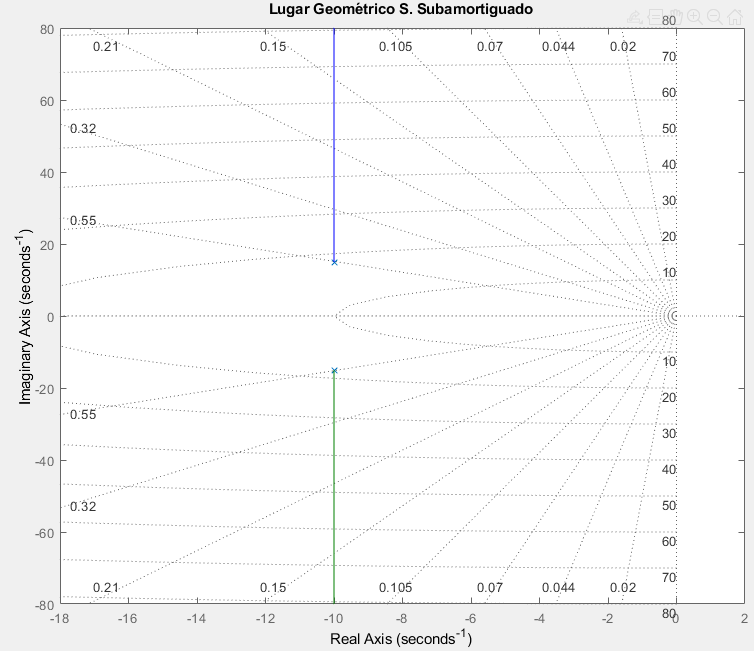
\includegraphics[width=0.4\textwidth]{media/lgr_planta}
		\caption{Lugar geométrico del sistema}
		\label{fig:lgrplanta}
	\end{figure}
	
	Y en la que se puede apreciar que la planta cuenta con 2 polos ubicados en $-10 \pm 15j$, del mismo se puede destacar que para tales polos se tiene un sobreimpulso del $12.3\%$, un valor de $\xi = 0.55$ a una frecuencia natural de $\omega_n = 18.02 [rads/s]$.
	
	Siendo así lo que se busca para este sistema la reducción del sobreimpulso del 12.3$\%$ al 6.18$\%$ (exactamente la mitad), aplicando para ello  compensadores en adelanto-atraso y su diseño mediante el lugar geométrico de las raíces, debido a la características del sistema para modelar la nueva respuesta del sistema se hará uso del polo dominante mediante el calculo de la nueva frecuencia natural y el factor de amortiguamiento, según las ecuaciones.
	\begin{equation}
		\xi = \frac{-\ln(\frac{M_p}{100})}{\sqrt{\ln(\frac{M_p}{100})^2 + \pi^2}}
		\label{eq:factor-amortiguamiento} 	
	\end{equation}
	
	\begin{equation}
		\omega_n = \frac{4}{\xi T_s}
		\label{eq:frecuencia-natural}
	\end{equation}
	
	\begin{equation}
		S_{1,2} = -\xi \omega_n \pm j\omega \sqrt{1-\xi^2}
		\label{eq:polos-deseados}
	\end{equation}
		
	Donde se destaca que: \\
	$M_p$ : Sobreimpulso \\
	$T_s$ : Tiempo de establecimiento\\
	
	Considerando un $M_p = 6.18\% $ y un $T_s = 0.5[s]$ el factor de amortiguamiento es: $\xi = 0.6638$ y la frecuencia natural $\omega_n = 12.05 [\frac{rads}{s}]$, siendo así que los polos dominantes según \ref{eq:polos-deseados} serán:
	\begin{equation}
		S_{1,2} = -8 \pm 9.012j
		\label{eq:polos-dominantes-sub}
	\end{equation}
	Una vez obtenidos estos polos será necesario comprobar si estos pertenecen al lugar geométrico de la planta/sistema, sin embargo al apreciar este modelamiento en la figura \ref{fig:lgrplanta} se puede confirmar que este polo deseado no pertenece al lugar geométrico es por ello será necesario calcular el angulo de compensación mediante la relación:
	
	\begin{equation}
		\theta_{cm} = 180 + \gamma - \theta_1 - \theta_2
		\label{eq:angulo-compensacion}
	\end{equation}
	
	En donde $\gamma$ es el angulo debido al cero del compensador y $\theta_1$, $\theta_2$ los ángulos formados entre los polos del sistema y el polo deseado, además para facilitar el calculo del compensador en adelanto se toma como criterio de diseño tomar el cero del compensador en el punto $s = -10$, lo cual nos facilitara el calculo directo del polo del compensador en función del angulo de compensación $\theta_{cm}$.
	
	Para $\gamma, \theta_1, \theta_2$ se tiene que:
	
	\begin{align}
		\gamma &= \arctan(\frac{9}{2}) = 77.47 \\
		\theta_1 &= \arctan(\frac{24}{2}) = 85.23 \\
		\theta_2 &= 180 - \arctan(\frac{6}{2}) = 108.43\\
	\end{align}
	
	Para finalmente tener el siguiente angulo $\theta_{cm}$
	\begin{align}
		\theta_{cm} &= 180 + 77.47 - 85.23 - 108.43 \\
		\theta_{cm} &= 63.81 \label{eq:angulo-compensacion-adelanto}
	\end{align}
	
	Y finalmente para el calculo del polo se considera la distante entre la parte real del polo deseado y la parte imaginaria del mismo sobre la tangente del angulo $\theta_{cm}$, obteniendo que el polo en $s = -12.45$, debido a la relación constituida en \ref{eq:polo-comp-adelanto}
	
	\begin{align}
		P_c = -8 -(\frac{9}{tan(63.81)})\\
		P_c = -12.42
		\label{eq:polo-comp-adelanto} 
	\end{align}
	
	Luego de ello será necesario calcular la ganancia del compensador $k_c$en adelanto, para ello se hace uso de la condición de magnitud, definida \ref{eq:}
	\begin{equation}
		k_c|G_c(s)|*|G(s)| = 1
		\label{eq:condicion-magnitud}
	\end{equation}
	Obteniendo un $k_c = 0.5086$ y finalmente el compensador en adelanto será: 
	\begin{equation}
		G_c(s) = 0.5086*\frac{s + 10}{s + 12.42}
	\end{equation}
	
	Mediante este compensador el sistema logra reducir el sobreimpulso, sin embargo se aprecia un pequeño atenuación, por lo que para corregir esto se agrega un compensador en atraso para corregir la respuesta, para el diseño del compensador se toma como criterio de diseño alejar los más posible el cero para que no tenga efecto sobre el sistema y se debe acercar el polo lo más posible para que sea considerado como un integrador, permitiendo modificar la respuesta a lo requerido, bajo estas consideraciones, se tiene que el polo se ubicara en $b = 0.0002$ y para el cero se multiplicara por un factor de 20 al valor real del polo deseado, obteniendo $a = 20*8 = 160$.
	
	Con el polo y cero definido la ganancia del compensador en atraso se define mediante \ref{eq:condicion-magnitud} con el agregado de que se considera en esta relación la ganancia del compensador en adelanto, siendo la ganancia del compensador $k_a = 0.0792$
	
	
	Con estos valores el compensador en atraso, es:
	\begin{equation}
		G_atr(s) = 0.0792*\frac{s + 160}{s + 0.0002}
		\label{eq:compensador-atraso-sub}
	\end{equation}
	
	Una vez definidos ambos compensadores el sistema compensado será:
	
	\begin{equation}
		G(s) = 0.5086*\frac{s + 10}{s + 12.42} *0.0792\frac{s + 160}{s + 0.0002}*\frac{325}{s^2 + 20s + 325}
		\label{eq:sistema-sub-compensado}	
	\end{equation}
	
	Sin embargo solo con esta compensación no se puede llegar al comportamiento deseado, es por ello que se hace uso del amplificador operacional $U_3$ el cual define una ganancia adicional al sistema y mediante la cual se logro adecuar al sistema para que tenga un sobrepico del 6.17\$ el cual es muy cercano al valor teórico definido.
	
	El sistema final, tendrá la siguiente forma considerando una ganancia adicional de 1.36.
	
	\begin{equation}
		G(s) = 0.05478*\frac{s + 10}{s + 12.42}*\frac{s + 160}{s + 0.0002}*\frac{325}{s^2 + 20s + 325}
		\label{eq:sistema-sub-compensado-final}	
	\end{equation}
	
	\subsection{\textbf{Caso Sobreamortiguado}}
	
	En el caso del sistema sobreamortiguado se busca reducir el tiempo de establecimiento a por lo menos la mitad y para ello se hará uso del procedimiento realizado en el caso previo y mediante el cual se compensará el sistema teniendo en cuenta nuevas consideraciones para la asignación de polo y ceros para los compensadores adelanto-atraso.
	
	El sistema para el sistema sobreamortiguado se define en \ref{eq:planta-sobre}
	
	\begin{equation}
		G(s) = \frac{440.75}{s^2 + 42s + 440.75}
		\label{eq:planta-sobre}
	\end{equation}
	
	Y al graficar el lugar geométrico mostrado en la figura \ref{fig:lgr-planta-sobre} se puede apreciar que este sistema tiene ambas raíces en el eje real en los puntos $P = -21.5$ y $P = -20.5$, además como lo requerido es disminuir el tiempo de establecimiento se puede hacer uso de las ecuaciones \ref{eq:factor-amortiguamiento}, \ref{eq:frecuencia-natural} para determinar los valores de $\xi$ adecuados para este propósito.
	
	\begin{figure}[h]
		\centering
		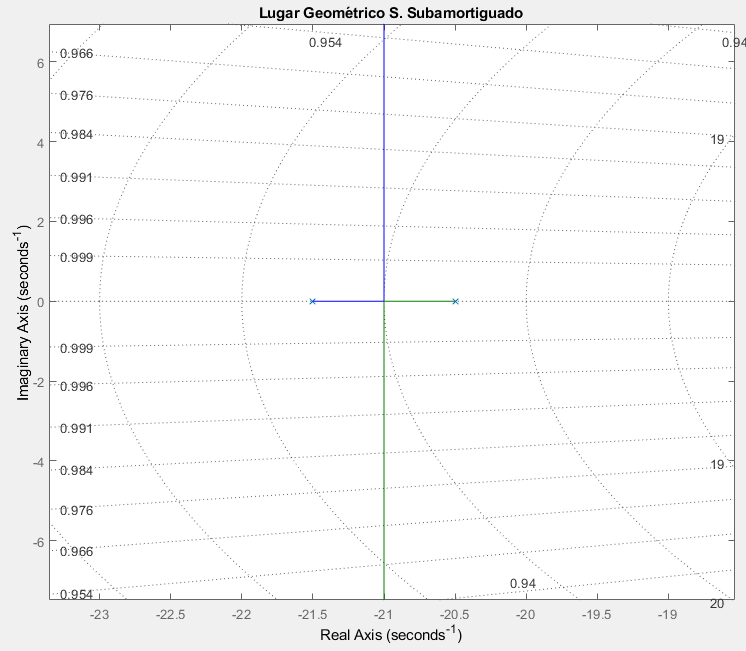
\includegraphics[width=0.4\textwidth]{media/lgr-planta-sobre}
		\caption{Lugar Geométrico del sistema sobreamortiguado}
		\label{fig:lgr-planta-sobre}
	\end{figure}
	
	En primera instancia el tiempo de establecimiento del sistema es de 0.38s por lo que se busca es reducir este tiempo a la mitad siendo el nuevo $T_s = 0.19s$ y al establecer un factor $\xi = 0.8$ se tiene una frecuencia natural $\omega_n = 26.3157$ que depende completamente del valor del tiempo de establecimiento.
	
	Una vez definidos estos parámetros se procede a calcular el polo deseado mediante \ref{eq:polos-deseados}, obteniendo la siguiente relación vista en: 
	
	\begin{equation}
		S_{1, 2} = -21.05 \pm 15.78i
		\label{eq:polos-deseados-sobre}
	\end{equation}
	
	De \ref{eq:polos-deseados-sobre} se puede apreciar en la figura \ref{fig:lgr-planta-sobre} que este polo no pertenece al LGR, por lo que será necesario calcular el angulo de compensación mediante la formula \ref{eq:angulo-compensacion} siendo esta equivalente a $\theta_{cm} = 4.95$ luego de restar el angulo de polos y ceros formados por el compensador y los polos de la planta.
	
	Este resultado es de esperarse debido a que para obtener una reducción en el tiempo de establecimiento el angulo de compensación se encuentra entre los 0 y 5 grados según los procesos experimentales, obteniendo el cero en a = 190 y el polo b = 203.1 ello para una ganancia $k_c = 0.6096$ luego de aplicar la condición de módulo para este compensador, finalmente este se modela como:
	
	\begin{equation}
		G_c(S) = 0.609*\frac{s + 190}{s + 203.1}
	\end{equation}
	
	Y finalmente para el compensador en atraso se considero un cero cercano al polo del sistema más apegado al eje semi-positivo del plano imaginario obteniendo una buena respuesta y para ajustar la respuesta del sistema se considero un polo cercano al origen y en relación al factor $\beta = 100$ el cual define que tan alejado se debe encontrar el polo del cero.
	
	Al tener en cuenta estas consideraciones y al aplicar la condición de módulo para la ganancia del compensador de atraso, este resultará $k_a = 1.1854$ con el cual se definirá el compensador en atraso el cual tendrá la siguiente forma.
	
	\begin{equation}
		G_{atr}(s) = 1.1854*\frac{s + 5.5}{s + 0.055}
		\label{eq:compensador-atr-sobre}
	\end{equation}
	
	Y el sistema aplicando los 2 compensadores a la planta original, tendrá la siguiente expresión:
	\begin{equation}
		G(s) = 0.609*\frac{s + 190}{s + 203.1}*1.1854*\frac{s + 5.5}{s + 0.055}*\frac{440.75}{s^2 + 42s + 440.75}
		\label{eq:compensador-adelanto-atr-sobre}
	\end{equation}
	
	Y de igual forma con tan solo estos compensadores no es posible obtener una respuesta adecuada es por ello que se hace uso de la ganancia externa definida en $U_3$ la cual nos permitirá reducir el tiempo de establecimiento a 0.19 para una ganancia de 100.
	
	\section{Usando el software Matlab, simule el sistema de control en lazo cerrado diseñado}
	Para la simulación de ambos sistemas,se hizo uso código MATLAB el cual permitió dinamizar el proceso de diseño al permitir el calculo de las diferentes respuestas del sistema al variar uno o varios parámetros, para el caso del sistema subamortiguado el código se muestra en:
	
	\begin{lstlisting}[numbers=none]
		clear, clc;
		
		% PLANTA
		num = [325];
		den = [1 20 325];
		planta  = tf(num, den);
		% Valores de compensacion
		mp = 6.18; % Reducir el sobrepico
		xi = -log(mp/100)/(sqrt(log(mp/100)^2 + pi^2));
		disp(["Xi: ", xi]);
		ts = 0.5; % Tiempo de establecimiento [s]
		wn = 4/(xi*ts);
		disp(["Freq Natural: ", wn]);
		raices_den = roots(den);
		
		% POLO DESEADO
		po = raices_den(1);
		
		disp(["Polos Sistema: ",po]);
		ps = -xi*wn + wn*sqrt(1-xi^2)*i;
		
		disp(["Polo deseado: ", ps]);
		
		% ================== COMPENSADOR ADELANTO ====================
		theta1 = atan((imag(ps)+imag(po))/(abs(real(po)) - abs(real(ps))))*180/pi;
		theta2 = 180 - atan( (imag(po) - imag(ps)) / (abs(real(po)) - abs(real(ps))))*180/pi;
		theta3 = atan(imag(ps)/(abs(real(po)) - abs(real(ps))))*180/pi;
		theta_com = 180 + theta3 - theta1 - theta2;
		disp(["Ang. Comp: ", theta_com]);
		
		cero_com = [1, -real(po)];
		polo_com = [1, -real(ps) + imag(ps)/(tan(theta_com*pi/180))];
		
		% Ganancia del compensador Kc
		kc = abs(evalfr(tf(conv(den, polo_com), conv(num, cero_com)), ps));
		disp(["Gan. Comp. Adelanto: ", kc]);
		
		% FUNCION DE TRANSFERENCIA DEL COMPENSADOR EN ADELANTO
		Gc = tf(cero_com, polo_com);
		Gc
		planta
		
		% ================== COMPENSADOR ATRASO ====================
		cero_catr = [1 -real(ps)*20];
		polo_catr = [1 0.0002];
		
		ka = abs(evalfr(tf( conv(conv(polo_catr,polo_com), den), conv(num*kc*cero_com,cero_catr)), ps));
		disp(["Gan. Comp. Atr: ", ka]);
		
		% FUNCION DE TRANSFERENCIA DEL COMPENSADOR EN ATRASO
		Gatr = tf(cero_catr, polo_catr);
		Gatr
		
		k=1.36;
		kt = kc*ka*k
		% LGR DEL SISTEMA
		sys_comp = tf( conv(kt*cero_catr,conv(cero_com, num)), conv(polo_catr, conv(polo_com,den)));
		sys_comp
		% rlocus(sys_comp);
		
		
		% Graficando la respuesta del sistema
		figure;
		sys_comp_retro = feedback(sys_comp, 1);
		tiempo_simulacion = 2;
		subplot(2, 1, 1);
		[resp_escalon_comp, t_escalon] = step(sys_comp_retro, tiempo_simulacion);
		plot(t_escalon, resp_escalon_comp, 'b', 'DisplayName', 'Sistema Compensado');
		hold on;
		[resp_escalon_planta, t_escalon] = step(planta, tiempo_simulacion);
		plot(t_escalon, resp_escalon_planta, 'r', 'DisplayName', 'Planta');
		
		title('Respuesta al Escalon Unitario - Subamortiguado');
		xlabel('Tiempo (s)');
		ylabel('Amplitud');
		legend show;
		grid on; 
		hold off;
		
		% Subgrafica 2: Respuesta al impulso 
		subplot(2, 1, 2); 
		[resp_impulso_comp, t_escalon] = impulse(sys_comp_retro, tiempo_simulacion);
		plot(t_escalon, resp_impulso_comp, 'b', 'DisplayName', 'Sistema Compensado');
		hold on;
		[resp_impulso_planta, t_escalon] = impulse(planta, tiempo_simulacion);
		plot(t_escalon, resp_impulso_planta, 'r', 'DisplayName', 'Planta');
		
		title('Respuesta al Impulso Unitario  - Subamortiguado');
		xlabel('Tiempo (s)');
		ylabel('Amplitud'); 
		legend show;
		grid on; 
		hold off;		% Agregar titulo general 
		sgtitle('Respuestas Sistema subamortiguado con Retroalimentacion Unitaria');
	\end{lstlisting}
	Para el caso del sistema sobreamortiguado el código MATLAB se vio modificado debido a que el calculo de los ángulos por polo y zero ven alteradas debido a la ubicación de estos en la plano complejo, siendo el código el mostrado acontinuación.
	
	\begin{lstlisting}[numbers=none]
		clear, clc;
		
		% PLANTA
		num = [440.75];
		den = [1 42 440.75];
		planta  = tf(num, den);
		% Valores de compensacion
		xi = 0.8;
		ts = 0.19; % Reducir ts
		disp(["Xi: ", xi]);
		wn = 4/(xi*ts);
		disp(["Freq Natural: ", wn]);
		po = roots(den);
		disp("Polos Sistema: ")
		disp(po);
		
		% POLO DESEADO
		ps = -xi*wn + wn*sqrt(1-xi^2)*i;
		
		disp(["Polo deseado: ", ps]);
		
		% ================== COMPENSADOR ADELANTO ====================
		theta1 = 180 - atan(imag(ps)/( abs(real(ps)) - abs(po(2)) ))*180/pi;
		theta2 = atan( imag(ps)/ ( abs(po(1)) - abs(real(ps)) ) )*180/pi;
		distancia = 190;
		theta3 = atan(imag(ps)/( distancia - abs(real(ps)) ))*180/pi;
		theta_com = 180 + theta3 - theta1 - theta2;
		disp(["Ang. Comp: ", theta_com]);
		
		cero_com = [1, distancia];
		polo_com = [1, -real(ps) + imag(ps)/(tan( theta_com*pi/180 )) ];
		
		% Ganancia del compensador Kc
		kc = abs(evalfr(tf(conv(den, polo_com), conv(num, cero_com)), ps));
		disp(["Gan. Comp. Adelanto: ", kc]);
		
		% FUNCION DE TRANSFERENCIA DEL COMPENSADOR EN ADELANTO
		Gc = tf(cero_com, polo_com);
		Gc
		planta
		
		% ================== COMPENSADOR ATRASO ====================
		beta = 100;
		cero = 15;
		cero_catr = [1, -po(2)-cero];
		polo_catr = [1, (-po(2)-cero)/beta];
		
		ka = abs(evalfr(tf( conv(conv(polo_catr,polo_com), den), conv(num*kc*cero_com,cero_catr)), ps));
		disp(["Gan. Comp. Atr: ", ka]);
		
		% FUNCION DE TRANSFERENCIA DEL COMPENSADOR EN ATRASO
		Gatr = tf(cero_catr, polo_catr);
		Gatr
		
		k=100;
		kt = kc*ka*k
		% LGR DEL SISTEMA
		sys_comp = tf( conv(kt*cero_catr,conv(cero_com, num)), conv(polo_catr, conv(polo_com,den)));
		sys_comp
		% rlocus(sys_comp);
		
		
		% Graficando la respuesta del sistema
		figure;
		sys_comp_retro = feedback(sys_comp, 1);
		tiempo_simulacion = 2;
		subplot(2, 1, 1);
		[resp_escalon_comp, t_escalon] = step(sys_comp_retro, tiempo_simulacion);
		plot(t_escalon, resp_escalon_comp, 'b', 'DisplayName', 'Sistema Compensado');
		hold on;
		[resp_escalon_planta, t_escalon] = step(planta, tiempo_simulacion);
		plot(t_escalon, resp_escalon_planta, 'r', 'DisplayName', 'Planta');
		
		title('Respuesta al Escalon Unitario - Sobreamortiguado');
		xlabel('Tiempo (s)');
		ylabel('Amplitud');
		legend show;
		grid on; 
		hold off;
		
		% Subgrafica 2: Respuesta al impulso 
		subplot(2, 1, 2); 
		[resp_impulso_comp, t_escalon] = impulse(sys_comp_retro, tiempo_simulacion);
		plot(t_escalon, resp_impulso_comp, 'b', 'DisplayName', 'Sistema Compensado');
		hold on;
		[resp_impulso_planta, t_escalon] = impulse(planta, tiempo_simulacion);
		plot(t_escalon, resp_impulso_planta, 'r', 'DisplayName', 'Planta');
		
		title('Respuesta al Impulso Unitario  - Sobreamortiguado');
		xlabel('Tiempo (s)');
		ylabel('Amplitud'); 
		legend show;
		grid on; 
		hold off;
		% Agregar titulo general 
		sgtitle('Respuestas Sistema Sobreamortiguado con Retroalimentacion Unitaria');
	\end{lstlisting}
	
	\section{Mostrar las gráficas del ítem anterior, ¿Cuál es la explicación de estas graficas?}
	
	\subsection{Caso Subamortiguado}
	La repuesta para ambos casos, se puede apreciar en la figura \ref{fig:respuesta-sub}
	\begin{figure}[h]
		\centering
		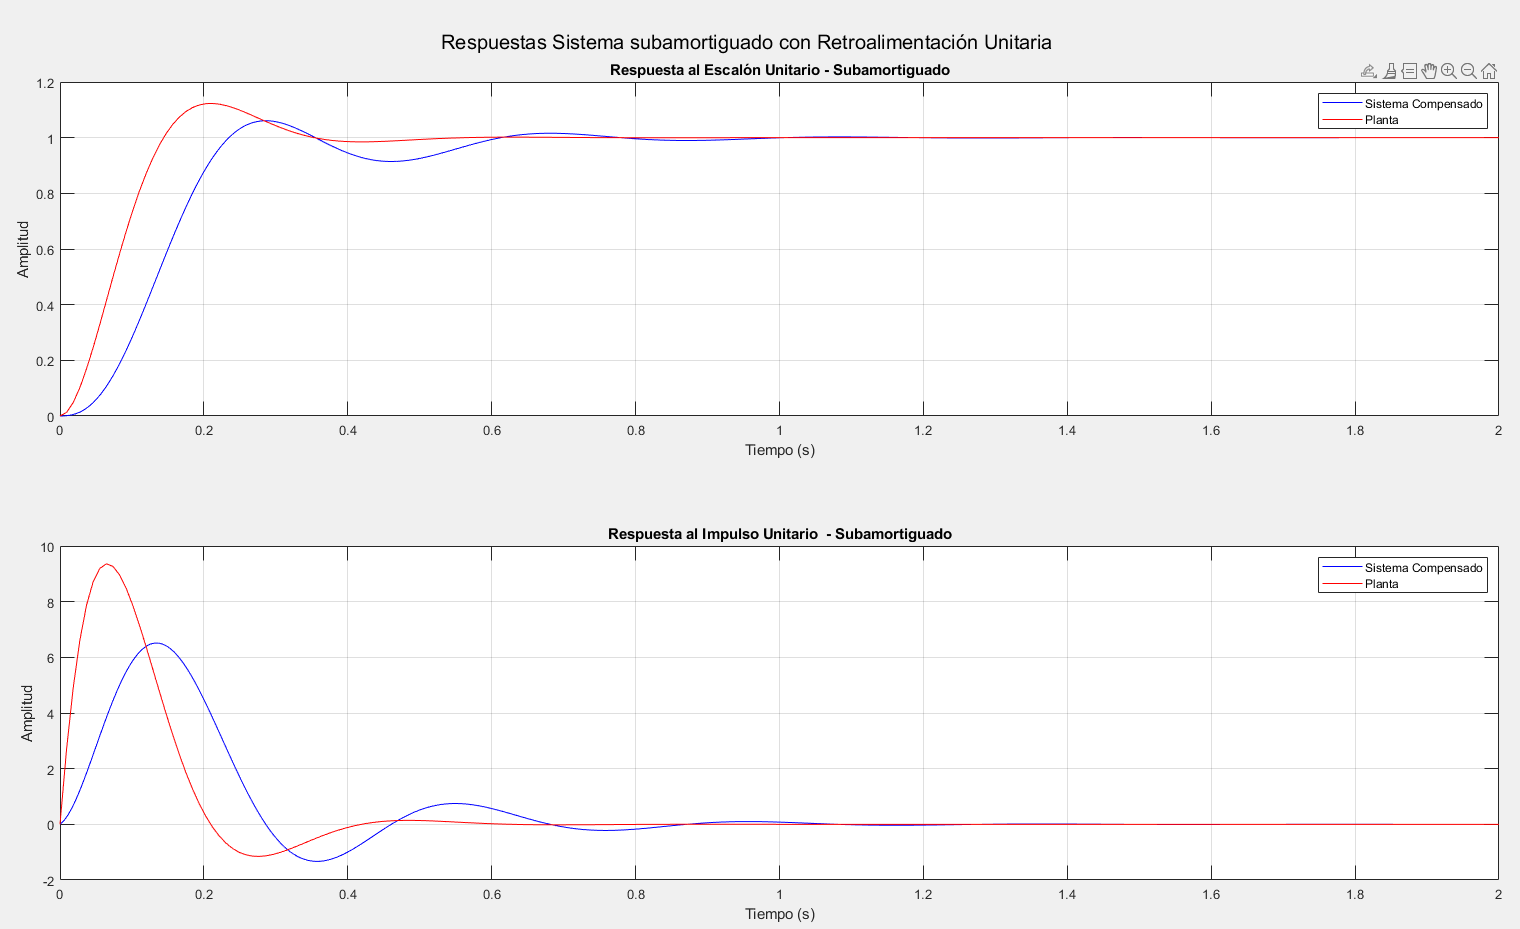
\includegraphics[width=0.5\textwidth]{media/respuesta-sub}
		\caption{Respuesta al escalón e impulso unitario del sistema subamortiguado}
		\label{fig:respuesta-sub}
	\end{figure}
	
	La figuras presentadas muestran la respuesta de un sistema de control en lazo cerrado a una entrada escalón unitario, en un caso subamortiguado, se observa claramente la presencia de oscilaciones alrededor del valor de estado estacionario, lo cual es característico de sistemas subamortiguados. El sobreimpulso, es decir, la máxima desviación de la salida respecto al valor de estado estacionario, es relativamente alto, lo que indica que el sistema presenta una cierta inestabilidad. El tiempo de asentamiento, el tiempo que tarda la salida en alcanzar y mantenerse dentro de una banda especificada alrededor del valor de estado estacionario, también parece ser relativamente largo. Estos resultados sugieren que el diseño del sistema de control podría requerir ajustes para mejorar su desempeño, como por ejemplo, aumentar el amortiguamiento del sistema.
	
	\subsection{Caso Sobreamortiguado}
	La respuesta para cada entrada se puede apreciar en la figura \ref{fig:respuesta-sobre}
	\begin{figure}[h]
		\centering
		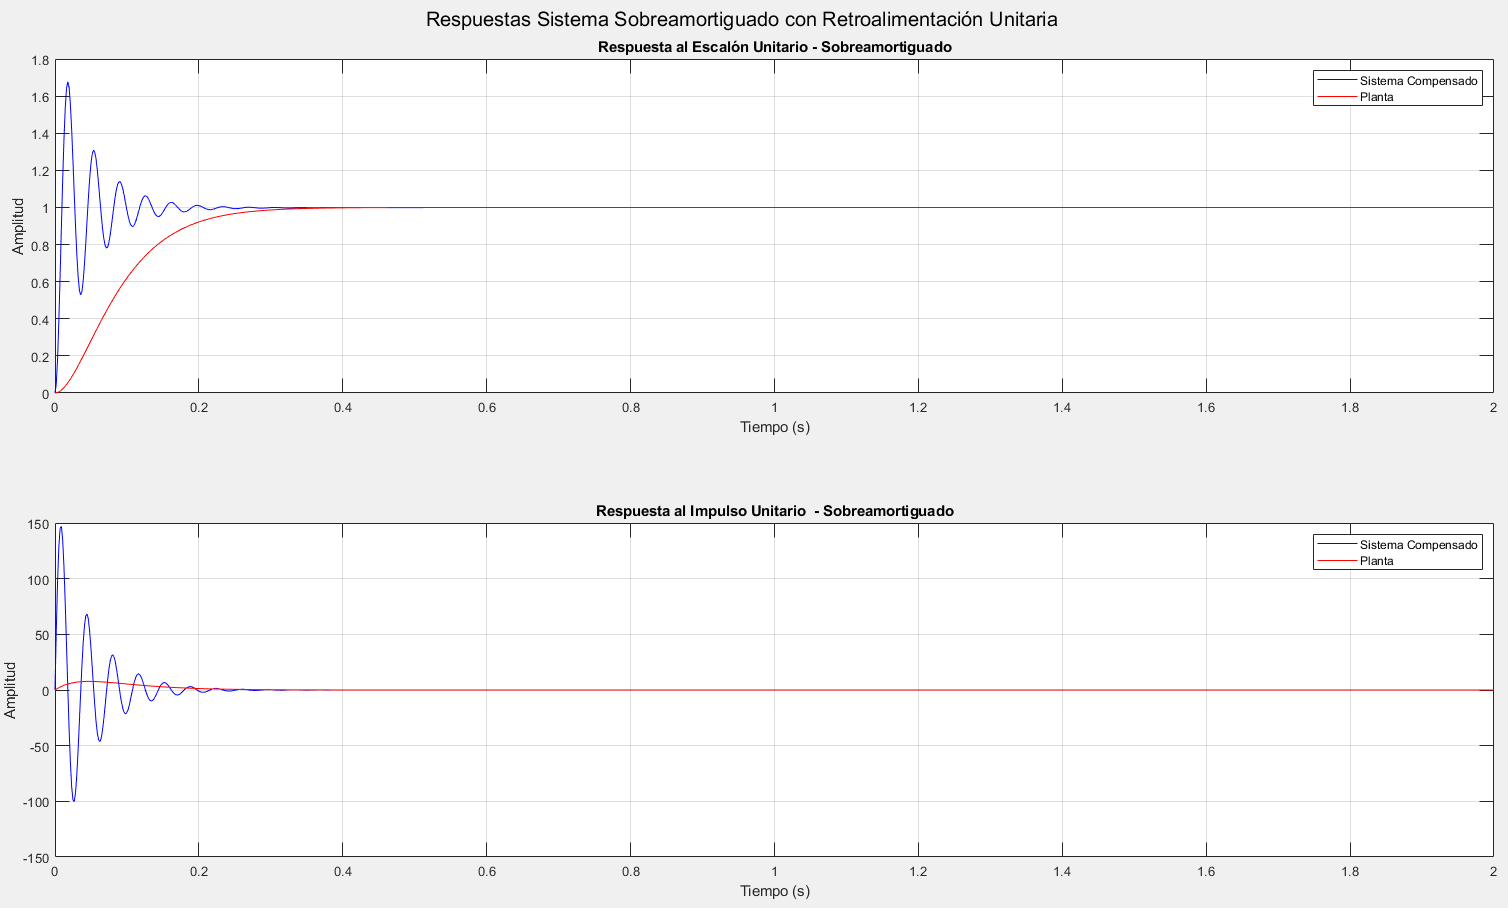
\includegraphics[width=0.5\textwidth]{media/respuesta-sobre}
		\caption{Respuesta al escalón e impulso del sistema sobreamortiguado}
		\label{fig:respuesta-sobre}
	\end{figure}
	
	\bibliographystyle{IEEEtran}
	\bibliography{biblio}
\end{document}



































